%%%%%%%%%%%%%%%%%%%%%%%%%%%%%%%%%%%%%%%%%%%%%%%%%%%%%%%%%%%%%%%%%%%%%%%%%%%%%%%%%
%%%%%                           ONLINE APPENDIX                              %%%%
%%%%%%%%%%%%%%%%%%%%%%%%%%%%%%%%%%%%%%%%%%%%%%%%%%%%%%%%%%%%%%%%%%%%%%%%%%%%%%%%%
%%%%%%%%%%%%%%%%%%%%%%%%%%%%%%%%%%%%%%%%%%%%%%%%%%%%%%%%%%%%%%%%%%%%%%%%%%%%%%%%%
\section{Appendix Tables}

\begin{table}[h!]
	\caption{Descriptive statistics of estimating panel: more variables}
	\label{tab:estimating_panel_stats_long}
	\centering
	
% Table created by stargazer v.5.2.2 by Marek Hlavac, Harvard University. E-mail: hlavac at fas.harvard.edu
% Date and time: Mon, Nov 30, 2020 - 11:59:19 AM
\begin{tabular}{@{\extracolsep{5pt}}lccccc} 
\\[-1.8ex]\hline 
\hline \\[-1.8ex] 
Statistic & \multicolumn{1}{c}{N} & \multicolumn{1}{c}{Mean} & \multicolumn{1}{c}{St. Dev.} & \multicolumn{1}{c}{Min} & \multicolumn{1}{c}{Max} \\ 
\hline \\[-1.8ex] 
Statutory MW & 156,600 & 8.08 & 1.21 & 7 & 16 \\ 
Experienced MW (total jobs) & 156,600 & 8.06 & 1.20 & 6.29 & 14.98 \\ 
Experienced MW (low inc.) & 156,600 & 8.06 & 1.20 & 5.81 & 15.02 \\ 
Experienced MW (young) & 156,600 & 8.06 & 1.20 & 6.19 & 15.07 \\ 
Median rent psqft. 2BR & 24,789 & 1.96 & 0.97 & 0.53 & 6.51 \\ 
Median rent psqft. MFR5plus & 37,588 & 1.96 & 1.05 & 0.55 & 6.69 \\ 
Median rent psqft.SFCC & 113,375 & 1.27 & 0.83 & 0.47 & 7.25 \\ 
Median rent SFCC & 125,644 & 1,651.10 & 702.99 & 595.00 & 6,595.00 \\ 
Avg. wage Fin. activities & 152,334 & 1,561.78 & 965.27 & 0.00 & 9,557.00 \\ 
Employment Fin. activities & 152,334 & 59,554.22 & 75,796.09 & 0.00 & 397,839.00 \\ 
Estab. count Fin. activities & 152,334 & 5,103.83 & 5,200.06 & 31.00 & 30,405.00 \\ 
Avg. wage Prof. and bus. serv. & 152,334 & 1,252.94 & 434.75 & 226.00 & 4,727.00 \\ 
Employment Prof. and bus. serv. & 152,334 & 134,280.40 & 143,863.40 & 329.00 & 640,795.00 \\ 
Estab. count Prof. and bus. serv. & 152,334 & 9,999.11 & 9,479.67 & 60.00 & 56,758.00 \\ 
Avg. wage Information & 152,334 & 1,505.07 & 619.82 & 0.00 & 7,380.00 \\ 
Employment Information & 152,334 & 21,041.80 & 35,131.53 & 0.00 & 238,776.00 \\ 
Estab. count Information & 152,334 & 920.54 & 1,381.95 & 4.00 & 13,271.00 \\ 
\hline \\[-1.8ex] 
\end{tabular} 

	\begin{minipage}{\textwidth} \footnotesize
		\vspace{3mm} 
		\textit{Notes}: The table shows summary statistics of our baseline estimating panel.
		Variables included are the statutory and experienced MW, constructed using different
		sets of weights as explained in \autoref{sec:mw_construction}; median monthly rents 
		per square foot in the categories 2 bedroom (2BR), multi family houses with 5 or more 
		units (MFR5plus), and SFCC, and absolute median rents for the SFCC category, all taken
		directly from Zillow; and average weekly wage, employment and establishment count 
		for three industries used in our estimation, obtained from the QCEW.
	\end{minipage}
\end{table}

\clearpage
\begin{table}[h!]
	\caption{Results from static model controlling for parametric trends}
	\label{tab:did_trend}
	\centering
	{
\def\sym#1{\ifmmode^{#1}\else\(^{#1}\)\fi}
\begin{tabular}{l*{6}{c}}
\hline\hline
          &\multicolumn{1}{c}{(1)}         &\multicolumn{1}{c}{(2)}         &\multicolumn{1}{c}{(3)}         &\multicolumn{1}{c}{(4)}         &\multicolumn{1}{c}{(5)}         &\multicolumn{1}{c}{(6)}         \\
\hline
$\Delta \ln \underline{w}_{ict}$&   0.0260\sym{**} &   0.0257\sym{**} &   0.0255\sym{**} &   0.0258\sym{**} &   0.0248\sym{**} &   0.0242\sym{**} \\
          & (0.0128)         & (0.0120)         & (0.0117)         & (0.0124)         & (0.0116)         & (0.0111)         \\
\hline
\vspace{-2mm}&                  &                  &                  &                  &                  &                  \\
Zipcode-specifc linear trend&       No         &      Yes         &      Yes         &       No         &      Yes         &      Yes         \\
Zipcode-specific quadratic trend&       No         &       No         &      Yes         &       No         &       No         &      Yes         \\
Local economy controls&       No         &       No         &       No         &      Yes         &      Yes         &      Yes         \\
R-squared &    0.022         &    0.024         &    0.026         &    0.022         &    0.024         &    0.027         \\
Observations&  112,232         &  112,232         &  112,232         &  107,814         &  107,814         &  107,814         \\
\hline\hline
\end{tabular}
}

	\begin{minipage}{0.95\textwidth} \footnotesize
		\vspace{3mm} 
		\textit{Notes}: The table reports coefficients from versions of \autoref{eq:did} 
		estimated on the balanced panel of zipcode-months described in \autoref{sec:data}. 
		The dependent variable is the difference in the natural logarithm of median	rents 
		per	square foot in the Single Family, Condos and Condominiums category in Zillow, 
		whereas the main independent variable is the difference in the natural logarithm
		of the statutory minimum wage. All columns include controls for monthly date fixed 
		effects. In addition, column (2) controls for zipcode-specific linear trend (which 
		in a differenced model amounts to including a zipcode fixed effect), and column (3) 
		controls for zipcode-specific linear and quadratic trends (which amount to including 
		a zipcode fixed effect and a zipcode-specific trend). Standard errors are clustered 
		at the state level. Significance codes: *** $p < 0.01$, ** $p < 0.05$, * $p < 0.1$.
	\end{minipage}
\end{table}

\clearpage
\begin{table}[h!]
	\caption{Complete results of dynamic model with leads and lags}
	\label{tab:dynamic_lags_leads_main}
	\centering
	{
\def\sym#1{\ifmmode^{#1}\else\(^{#1}\)\fi}
\begin{tabular}{l*{5}{c}}
\hline\hline
          &\multicolumn{1}{c}{(1)}         &\multicolumn{1}{c}{(2)}         &\multicolumn{1}{c}{(3)}         &\multicolumn{1}{c}{(4)}         &\multicolumn{1}{c}{(5)}         \\
\hline
$\Delta \ln \underline{w}_{ic,t-5}$&  -0.0148         &  -0.0144         &  -0.0144         &  -0.0146         &  -0.0144         \\
          & (0.0090)         & (0.0089)         & (0.0089)         & (0.0090)         & (0.0089)         \\
[1em]
$\Delta \ln \underline{w}_{ic,t-4}$&  -0.0024         &  -0.0019         &  -0.0020         &  -0.0022         &  -0.0019         \\
          & (0.0116)         & (0.0116)         & (0.0115)         & (0.0116)         & (0.0115)         \\
[1em]
$\Delta \ln \underline{w}_{ic,t-3}$&   0.0011         &   0.0005         &   0.0007         &   0.0004         &  -0.0002         \\
          & (0.0092)         & (0.0094)         & (0.0092)         & (0.0091)         & (0.0092)         \\
[1em]
$\Delta \ln \underline{w}_{ic,t-2}$&   0.0060         &   0.0063         &   0.0062         &   0.0060         &   0.0064         \\
          & (0.0116)         & (0.0118)         & (0.0116)         & (0.0115)         & (0.0117)         \\
[1em]
$\Delta \ln \underline{w}_{ic,t-1}$&  -0.0002         &  -0.0004         &  -0.0005         &   0.0000         &  -0.0005         \\
          & (0.0123)         & (0.0123)         & (0.0124)         & (0.0122)         & (0.0123)         \\
[1em]
$\Delta \ln \underline{w}_{ic,t}$&   0.0271\sym{**} &   0.0257\sym{**} &   0.0259\sym{**} &   0.0269\sym{**} &   0.0259\sym{**} \\
          & (0.0126)         & (0.0123)         & (0.0124)         & (0.0126)         & (0.0124)         \\
[1em]
$\Delta \ln \underline{w}_{ic,t+1}$&   0.0136\sym{*}  &   0.0146\sym{**} &   0.0142\sym{*}  &   0.0135\sym{*}  &   0.0146\sym{*}  \\
          & (0.0072)         & (0.0072)         & (0.0072)         & (0.0072)         & (0.0072)         \\
[1em]
$\Delta \ln \underline{w}_{ic,t+2}$&  -0.0070         &  -0.0066         &  -0.0064         &  -0.0068         &  -0.0064         \\
          & (0.0133)         & (0.0133)         & (0.0132)         & (0.0133)         & (0.0132)         \\
[1em]
$\Delta \ln \underline{w}_{ic,t+3}$&   0.0036         &   0.0045         &   0.0047         &   0.0031         &   0.0040         \\
          & (0.0081)         & (0.0078)         & (0.0078)         & (0.0079)         & (0.0077)         \\
[1em]
$\Delta \ln \underline{w}_{ic,t+4}$&   0.0108         &   0.0093         &   0.0104         &   0.0107         &   0.0096         \\
          & (0.0069)         & (0.0066)         & (0.0064)         & (0.0069)         & (0.0065)         \\
[1em]
$\Delta \ln \underline{w}_{ic,t+5}$&   0.0086         &   0.0095         &   0.0099         &   0.0088         &   0.0099         \\
          & (0.0069)         & (0.0065)         & (0.0065)         & (0.0067)         & (0.0065)         \\
\hline
\vspace{-2mm}&                  &                  &                  &                  &                  \\
Cumulative effect&    0.057         &0.057\sym{*}         &0.059\sym{*}         &    0.056         &0.058\sym{*}         \\
          &  (0.035)         &  (0.034)         &  (0.034)         &  (0.034)         &  (0.034)         \\
\hline    &                  &                  &                  &                  &                  \\
P-value no pretrends&    0.568         &    0.612         &    0.599         &    0.594         &    0.629         \\
Wage controls&       No         &      Yes         &       No         &       No         &      Yes         \\
Employment controls&       No         &       No         &      Yes         &       No         &      Yes         \\
Establishment-count controls&       No         &       No         &       No         &      Yes         &      Yes         \\
R-squared &    0.022         &    0.022         &    0.022         &    0.022         &    0.022         \\
Observations&  106,446         &  105,463         &  105,463         &  106,160         &  105,463         \\
\hline\hline
\end{tabular}
}

	\begin{minipage}{0.95\textwidth} \footnotesize
		\vspace{3mm} 
		\textit{Notes}: The table reports coefficients from versions of 
		\autoref{eq:leads_lags} estimated on the balanced panel of zipcode-months
		described in \autoref{sec:data}. The dependent variable is the difference in 
		the natural logarithm of median	rents per square foot in the Single Family, Condos 
		and Condominiums category in Zillow. We report coefficients of five leads and lags 
		of the difference in the logarithm of the statutory minimum wage. All columns 
		control for monthly date fixed effects. In addition, columns (2) to (5) include 
		economic controls from the industries ``Professional and business services'', 
		``Information'', and ``Financial activities'' from the QCEW. Wage controls are 
		the difference in the natural logarithm of average weekly wages, employment 
		controls are the difference in the natural logarithm of employment, and 
		establishment count controls refer to the difference in the natural logarithm 
		of number of establishments. Wages and employment vary at the county-month level,
		whereas establishment count varies at the country-quarter level. The row 
		``Cumulative Effect'' shows the cumulative 	sum of the sum of all coefficients. 
		Standard errors are clustered at the state level. Significance codes: *** $p < 
		0.01$, ** $p < 0.05$, * $p < 0.1$.
	\end{minipage}
\end{table}

\begin{table}[h!]\centering
	\caption{Complete results for static model, dynamic models, and panel models with 
		lagged dependent variable as control}
	\label{tab:horse_race_ab}
	\resizebox{.9\textwidth}{!}{
	{
\def\sym#1{\ifmmode^{#1}\else\(^{#1}\)\fi}
\begin{tabular}{l*{8}{c}}
\hline\hline
          &\multicolumn{1}{c}{(1)}&\multicolumn{1}{c}{(2)}&\multicolumn{1}{c}{(3)}&\multicolumn{1}{c}{(4)}&\multicolumn{1}{c}{(5)}&\multicolumn{1}{c}{(6)}&\multicolumn{1}{c}{(7)}&\multicolumn{1}{c}{(8)}\\
          &\multicolumn{1}{c}{DiD}&\multicolumn{1}{c}{Distributed leads and lags}&\multicolumn{1}{c}{Distributed Lags}&\multicolumn{1}{c}{AB distributed leads and lags}&\multicolumn{1}{c}{AB distributed lags}&\multicolumn{1}{c}{est6}&\multicolumn{1}{c}{est7}&\multicolumn{1}{c}{est8}\\
\hline
\Delta ln(MW)_{t-5}&                  &  -0.0146         &                  &  -0.0159         &  -0.0134         &                  &  -0.0167         &                  \\
          &                  &(0.00910)         &                  &(0.00991)         &(0.00910)         &                  & (0.0155)         &                  \\
[1em]
\Delta ln(MW)_{t-4}&                  & -0.00232         &                  & -0.00576         &  0.00494         &                  & -0.00886         &                  \\
          &                  & (0.0116)         &                  & (0.0129)         & (0.0105)         &                  & (0.0347)         &                  \\
[1em]
\Delta ln(MW)_{t-3}&                  &  0.00137         &                  &  0.00100         &  0.00222         &                  & 0.000503         &                  \\
          &                  &(0.00931)         &                  & (0.0106)         &(0.00918)         &                  & (0.0152)         &                  \\
[1em]
\Delta ln(MW)_{t-2}&                  &  0.00608         &                  &  0.00625         &  0.00581         &                  &  0.00647         &                  \\
          &                  & (0.0115)         &                  & (0.0107)         & (0.0139)         &                  & (0.0102)         &                  \\
[1em]
\Delta ln(MW)_{t-1}&                  &-0.000280         &                  & -0.00141         & -0.00531         &                  &-0.000132         &                  \\
          &                  & (0.0123)         &                  &(0.00995)         & (0.0151)         &                  & (0.0154)         &                  \\
[1em]
\Delta ln(MW)_{t}&   0.0259\sym{*}  &   0.0270\sym{**} &   0.0261\sym{*}  &   0.0269\sym{**} &   0.0294\sym{*}  &   0.0288\sym{*}  &   0.0267\sym{**} &   0.0256\sym{**} \\
          & (0.0129)         & (0.0127)         & (0.0129)         & (0.0111)         & (0.0157)         & (0.0160)         & (0.0104)         & (0.0106)         \\
[1em]
\Delta ln(MW)_{t+1}&                  &   0.0136\sym{*}  &   0.0161\sym{**} &   0.0205\sym{**} & 0.000887         &  0.00401         &   0.0267         &   0.0304         \\
          &                  &(0.00715)         &(0.00750)         &(0.00860)         &(0.00733)         &(0.00788)         & (0.0514)         & (0.0536)         \\
[1em]
\Delta ln(MW)_{t+2}&                  & -0.00702         & -0.00673         & -0.00389         &  -0.0131         &  -0.0142         & -0.00102         &  0.00170         \\
          &                  & (0.0133)         & (0.0125)         & (0.0138)         & (0.0128)         & (0.0120)         & (0.0286)         & (0.0354)         \\
[1em]
\Delta ln(MW)_{t+3}&                  &  0.00364         &  0.00392         &  0.00211         &  0.00651         &  0.00692         & 0.000616         & 0.000316         \\
          &                  &(0.00808)         &(0.00799)         &(0.00972)         &(0.00798)         &(0.00764)         & (0.0158)         & (0.0173)         \\
[1em]
\Delta ln(MW)_{t+4}&                  &   0.0108         &   0.0105         &   0.0112         &  0.00897         &  0.00850         &   0.0120         &   0.0122         \\
          &                  &(0.00693)         &(0.00684)         &(0.00737)         &(0.00736)         &(0.00737)         & (0.0108)         & (0.0119)         \\
[1em]
\Delta ln(MW)_{t+5}&                  &  0.00862         &  0.00637         &   0.0102         &  0.00384         &  0.00163         &   0.0124         &   0.0112         \\
          &                  &(0.00686)         &(0.00675)         &(0.00655)         &(0.00878)         &(0.00870)         & (0.0160)         & (0.0174)         \\
[1em]
\Delta ln(y)_{t-1}&                  &                  &                  &   -0.240\sym{***}&    0.421\sym{***}&    0.436\sym{***}&   -0.451         &   -0.531         \\
          &                  &                  &                  &(0.00646)         & (0.0238)         & (0.0231)         &  (1.634)         &  (1.812)         \\
\hline
Observations& 1.12e+05         & 1.06e+05         & 1.12e+05         & 1.05e+05         & 1.04e+05         & 1.10e+05         & 1.05e+05         & 1.11e+05         \\
\hline\hline
\end{tabular}
}

	}
	\begin{minipage}{\textwidth} \footnotesize
		\vspace{3mm} 
		\textit{Notes:} The table reports coefficients from versions of \autoref{eq:did} and
		\autoref{eq:leads_lags} estimated on the balanced panel of zipcode-months
		described in \autoref{sec:data}. The dependent variable is the difference in 
		the natural logarithm of median	rents per square foot in the Single Family, Condos 
		and Condominiums category in Zillow. Column 1, 2, and 3 reports the baseline
		DiD, dynamic and distributed-lags models respectively. Column 4 presents estimates
		for a dynamic model where we additionally control for the lagged values of the dependent 
		variable. The model is estimated following \textcite{ArellanoBond1991}, 
		where $\Delta \ln y_{ic, t-1}$ is instrumented with $\Delta \ln y_{ic, t-2}$. Column 5 
		replicates column 4 specification while restricting leads of changes in (log) MW to be zero.
		All columns control for monthly date fixed effects. All columns additionally  
		include economic controls from the industries ``Professional and business services'', 
		``Information'', and ``Financial activities'' from the QCEW. Wage controls are 
		the difference in the natural logarithm of average weekly wages, employment 
		controls are the difference in the natural logarithm of employment, and 
		establishment count controls refer to the difference in the natural logarithm 
		of number of establishments. Wages and employment vary at the county-month level,
		whereas establishment count varies at the country-quarter level. The row 
		``Cumulative Effect'' shows the cumulative 	sum of the sum of all coefficients. 
		Standard errors are clustered at the state level. Significance codes: *** $p < 0.01$, 
		** $p < 0.05$, * $p < 0.1$.
	\end{minipage}
\end{table}


%\clearpage
%\begin{table}[h!]
%    \caption{Comparison between unbalanced and baseline panel model estimation}
%    \label{tab:comparison_unbal_base}
%    \centering
%     \resizebox{\textwidth}{!}{
%    \vspace{0pt}    
%    {
\def\sym#1{\ifmmode^{#1}\else\(^{#1}\)\fi}
\begin{tabular}{l*{6}{c}}
\hline\hline
          &\multicolumn{3}{c}{Unbalanced Panel}                    &\multicolumn{3}{c}{Baseline Panel}                      \\\cmidrule(lr){2-4}\cmidrule(lr){5-7}
          &\multicolumn{1}{c}{(1)}&\multicolumn{1}{c}{(2)}&\multicolumn{1}{c}{(3)}&\multicolumn{1}{c}{(4)}&\multicolumn{1}{c}{(5)}&\multicolumn{1}{c}{(6)}\\
          &\multicolumn{1}{c}{DiD}&\multicolumn{1}{c}{\shortstack{Distributed \\ leads and lags}}&\multicolumn{1}{c}{\shortstack{Distributed \\ Lags}}&\multicolumn{1}{c}{DiD}&\multicolumn{1}{c}{\shortstack{Distributed \\ leads and lags}}&\multicolumn{1}{c}{\shortstack{Distributed \\ Lags}}\\
\hline
$\Delta \ln(MW)_{t-5}$&                  &  -0.0115         &                  &                  &  -0.0153         &                  \\
          &                  &(0.00810)         &                  &                  &(0.00915)         &                  \\
[1em]
$\Delta \ln(MW)_{t-4}$&                  & -0.00812         &                  &                  & -0.00306         &                  \\
          &                  &(0.00792)         &                  &                  & (0.0110)         &                  \\
[1em]
$\Delta \ln(MW)_{t-3}$&                  & -0.00171         &                  &                  & 0.000380         &                  \\
          &                  &(0.00864)         &                  &                  &(0.00829)         &                  \\
[1em]
$\Delta \ln(MW)_{t-2}$&                  & -0.00233         &                  &                  &  0.00531         &                  \\
          &                  &(0.00743)         &                  &                  & (0.0121)         &                  \\
[1em]
$\Delta \ln(MW)_{t-1}$&                  &  0.00552         &                  &                  &-0.000798         &                  \\
          &                  &(0.00823)         &                  &                  & (0.0126)         &                  \\
[1em]
$\Delta \ln(MW)_{t}$&   0.0220\sym{*}  &   0.0218\sym{*}  &   0.0229\sym{*}  &   0.0257\sym{**} &   0.0265\sym{**} &   0.0268\sym{**} \\
          & (0.0111)         & (0.0117)         & (0.0115)         & (0.0120)         & (0.0119)         & (0.0126)         \\
[1em]
$\Delta \ln(MW)_{t+1}$&                  &  0.00473         &  0.00788         &                  &   0.0128\sym{*}  &   0.0162\sym{*}  \\
          &                  &(0.00574)         &(0.00586)         &                  &(0.00739)         &(0.00816)         \\
[1em]
$\Delta \ln(MW)_{t+2}$&                  &  0.00405         &  0.00558         &                  & -0.00785         & -0.00623         \\
          &                  &(0.00915)         &(0.00772)         &                  & (0.0135)         & (0.0128)         \\
[1em]
$\Delta \ln(MW)_{t+3}$&                  &  0.00347         &  0.00638         &                  &  0.00277         &  0.00359         \\
          &                  &(0.00632)         &(0.00636)         &                  &(0.00751)         &(0.00830)         \\
[1em]
$\Delta \ln(MW)_{t+4}$&                  &  0.00515         &  0.00505         &                  &  0.00994         &   0.0108         \\
          &                  &(0.00688)         &(0.00684)         &                  &(0.00695)         &(0.00704)         \\
[1em]
$\Delta \ln(MW)_{t+5}$&                  & 0.000767         & -0.00261         &                  &  0.00778         &  0.00641         \\
          &                  &(0.00774)         &(0.00800)         &                  &(0.00735)         &(0.00691)         \\
\hline
Observations&   194295         &   177659         &   194209         &   112232         &   106446         &   112161         \\
\hline\hline
\end{tabular}
}

%    }
%    \begin{minipage}{.95\textwidth} \footnotesize
%		\vspace{3mm} 
%		\textit{Notes}: The table compares estimates from our main specifications (\textit{static DiD}, 
%		\textit{distributed leads and lags DiD}, and \textit{distributed lags DiD}) obtained using the 
%		baseline sample with estimates obtained using the unbalanced, full sample of zipcodes. Columns 
%		(1), (2), and (3) show results from from \autoref{eq:did}, (\ref{eq:leads_lags}), and (\ref{eq:lags}) 
%		respectively, using the unbalanced sample. All three columns additionally control for ``cohort 
%		$\times$ period" FE to account for differences in the each zipcodes time series. Columns (4), (5), 
%		and (6) replicates our main results obtained with the baseline sample and presented in 
%		\autoref{tab: did_main}, column (2), \autoref{tab: dynamic_lags_leads_main}, column (2) and 
%		\autoref{tab:horse_race_main}. All specifications control for zipcode-level linear trends. 
%		Standard errors clustered at the state level. *** $p < 0.01$, ** $p < 0.05$, * $p < 0.1$.  
%	\end{minipage}
%\end{table}

%\clearpage
%\begin{table}[h!]
%    \caption{Comparison between baseline and re-weighted panel model estimation}
%    \label{tab:comparison_wgt_base}
%    \centering
%    \resizebox{\textwidth}{!}{
%	    \vspace{0pt}    
%	    {
\def\sym#1{\ifmmode^{#1}\else\(^{#1}\)\fi}
\begin{tabular}{l*{6}{c}}
\hline\hline
          &\multicolumn{3}{c}{Reweighted Panel}                    &\multicolumn{3}{c}{Baseline Panel}                      \\\cmidrule(lr){2-4}\cmidrule(lr){5-7}
          &\multicolumn{1}{c}{(1)}&\multicolumn{1}{c}{(2)}&\multicolumn{1}{c}{(3)}&\multicolumn{1}{c}{(4)}&\multicolumn{1}{c}{(5)}&\multicolumn{1}{c}{(6)}\\
          &\multicolumn{1}{c}{DiD}&\multicolumn{1}{c}{\shortstack{Distributed \\ leads and lags}}&\multicolumn{1}{c}{\shortstack{Distributed \\ Lags}}&\multicolumn{1}{c}{DiD}&\multicolumn{1}{c}{\shortstack{Distributed \\ leads and lags}}&\multicolumn{1}{c}{\shortstack{Distributed \\ Lags}}\\
\hline
$\Delta \ln(MW)_{t-5}$&                  & -0.00832         &                  &                  &  -0.0153         &                  \\
          &                  &(0.00687)         &                  &                  &(0.00915)         &                  \\
[1em]
$\Delta \ln(MW)_{t-4}$&                  &  0.00566         &                  &                  & -0.00306         &                  \\
          &                  &(0.00726)         &                  &                  & (0.0110)         &                  \\
[1em]
$\Delta \ln(MW)_{t-3}$&                  &  0.00821         &                  &                  & 0.000380         &                  \\
          &                  &(0.00905)         &                  &                  &(0.00829)         &                  \\
[1em]
$\Delta \ln(MW)_{t-2}$&                  &-0.000403         &                  &                  &  0.00531         &                  \\
          &                  & (0.0115)         &                  &                  & (0.0121)         &                  \\
[1em]
$\Delta \ln(MW)_{t-1}$&                  & -0.00860         &                  &                  &-0.000798         &                  \\
          &                  & (0.0116)         &                  &                  & (0.0126)         &                  \\
[1em]
$\Delta \ln(MW)_{t}$&   0.0365\sym{***}&   0.0369\sym{***}&   0.0372\sym{***}&   0.0257\sym{**} &   0.0265\sym{**} &   0.0268\sym{**} \\
          & (0.0124)         & (0.0127)         & (0.0132)         & (0.0120)         & (0.0119)         & (0.0126)         \\
[1em]
$\Delta \ln(MW)_{t+1}$&                  &  0.00782         &  0.00942         &                  &   0.0128\sym{*}  &   0.0162\sym{*}  \\
          &                  &(0.00706)         &(0.00730)         &                  &(0.00739)         &(0.00816)         \\
[1em]
$\Delta \ln(MW)_{t+2}$&                  & -0.00822         & -0.00694         &                  & -0.00785         & -0.00623         \\
          &                  & (0.0167)         & (0.0160)         &                  & (0.0135)         & (0.0128)         \\
[1em]
$\Delta \ln(MW)_{t+3}$&                  &  0.00560         &  0.00516         &                  &  0.00277         &  0.00359         \\
          &                  &(0.00600)         &(0.00693)         &                  &(0.00751)         &(0.00830)         \\
[1em]
$\Delta \ln(MW)_{t+4}$&                  &   0.0100         &   0.0103         &                  &  0.00994         &   0.0108         \\
          &                  &(0.00939)         &(0.00935)         &                  &(0.00695)         &(0.00704)         \\
[1em]
$\Delta \ln(MW)_{t+5}$&                  &  0.00798         &  0.00781         &                  &  0.00778         &  0.00641         \\
          &                  &(0.00808)         &(0.00870)         &                  &(0.00735)         &(0.00691)         \\
\hline
Observations&  112,232         &  106,446         &  112,161         &  112,232         &  106,446         &  112,161         \\
\hline\hline
\end{tabular}
}

%    }
%    \begin{minipage}{.95\textwidth} \footnotesize
%		\vspace{3mm} 
%		\textit{Notes}: The table compares estimates from our main specifications (\textit{static 
%		DiD}, \textit{distributed leads and lags DiD}, and \textit{distributed lags DiD}) obtained 
%		using the baseline sample with estimates obtained using the reweighted sample (see 
%		\autoref{sec:sample_rest} for more details on how the weights are built). Columns (1), (2), 
%		and (3) show results from from \autoref{eq:did}, (\ref{eq:leads_lags}), and (\ref{eq:lags}) 
%		respectively, using the unbalanced sample. All three columns additionally control for 
%		``cohort $\times$ period" FE to account for differences in the each zipcodes time series. 
%		Columns (4), (5), and (6) replicates our main results obtained with the baseline sample 
%		and presented in \autoref{tab: did_main}, column (2), \autoref{tab: dynamic_lags_leads_main}, 
%		column (2) and \autoref{tab:horse_race_main}. All specifications control for zipcode-level 
%		linear trends. Standard errors clustered at the state level. *** $p < 0.01$, ** $p < 0.05$, 
%		* $p < 0.1$.
%	\end{minipage}
%\end{table}

\clearpage
%%%%%%%%%%%%%%%%%%%%%%%%%%%%%%%%%%%%%%%%%%%%%%%%%%%%%%%%%%%%%%%%%%%%%%%%%%%%%%%%%
\section{Appendix Figures}

\begin{figure}[!h]
	\centering
	\caption{National Time Series for Zillow and SAFMR data}
	\label{fig:trend_zillow_safmrwgt}
	\includegraphics[width = 0.7\textwidth]{../../analysis/zillow_benchmark/output/trend_zillow_safmrwgt_zipcode_avg.eps}
	\begin{minipage}{0.95\textwidth} \footnotesize
		\vspace{3mm}
		\textit{Notes:} The figure plots the annual national average for median	rents in the Single 
		Family, Condos and Condominiums category in Zillow, and a weighted combination of SAFMR series 
		with different number of bedrooms. Weights are based on the US share of single family, 
		condos and cooperative houses with given number of bedrooms as recorded in the \textit{American Housing 
		Survey} (\href{https://www.census.gov/programs-surveys/ahs.html}{AHS}). $\rho = 94.06$ percent. 
		See footnote \ref{foot:zillow_time_series} for details on the construction of this time series.  
	\end{minipage}
\end{figure}

\begin{figure}
	\caption{Comparison Between Zillow Sample and Population Density in CBSAs}
	\label{fig:maps}
	\begin{subfigure}[b]{\textwidth}\centering
		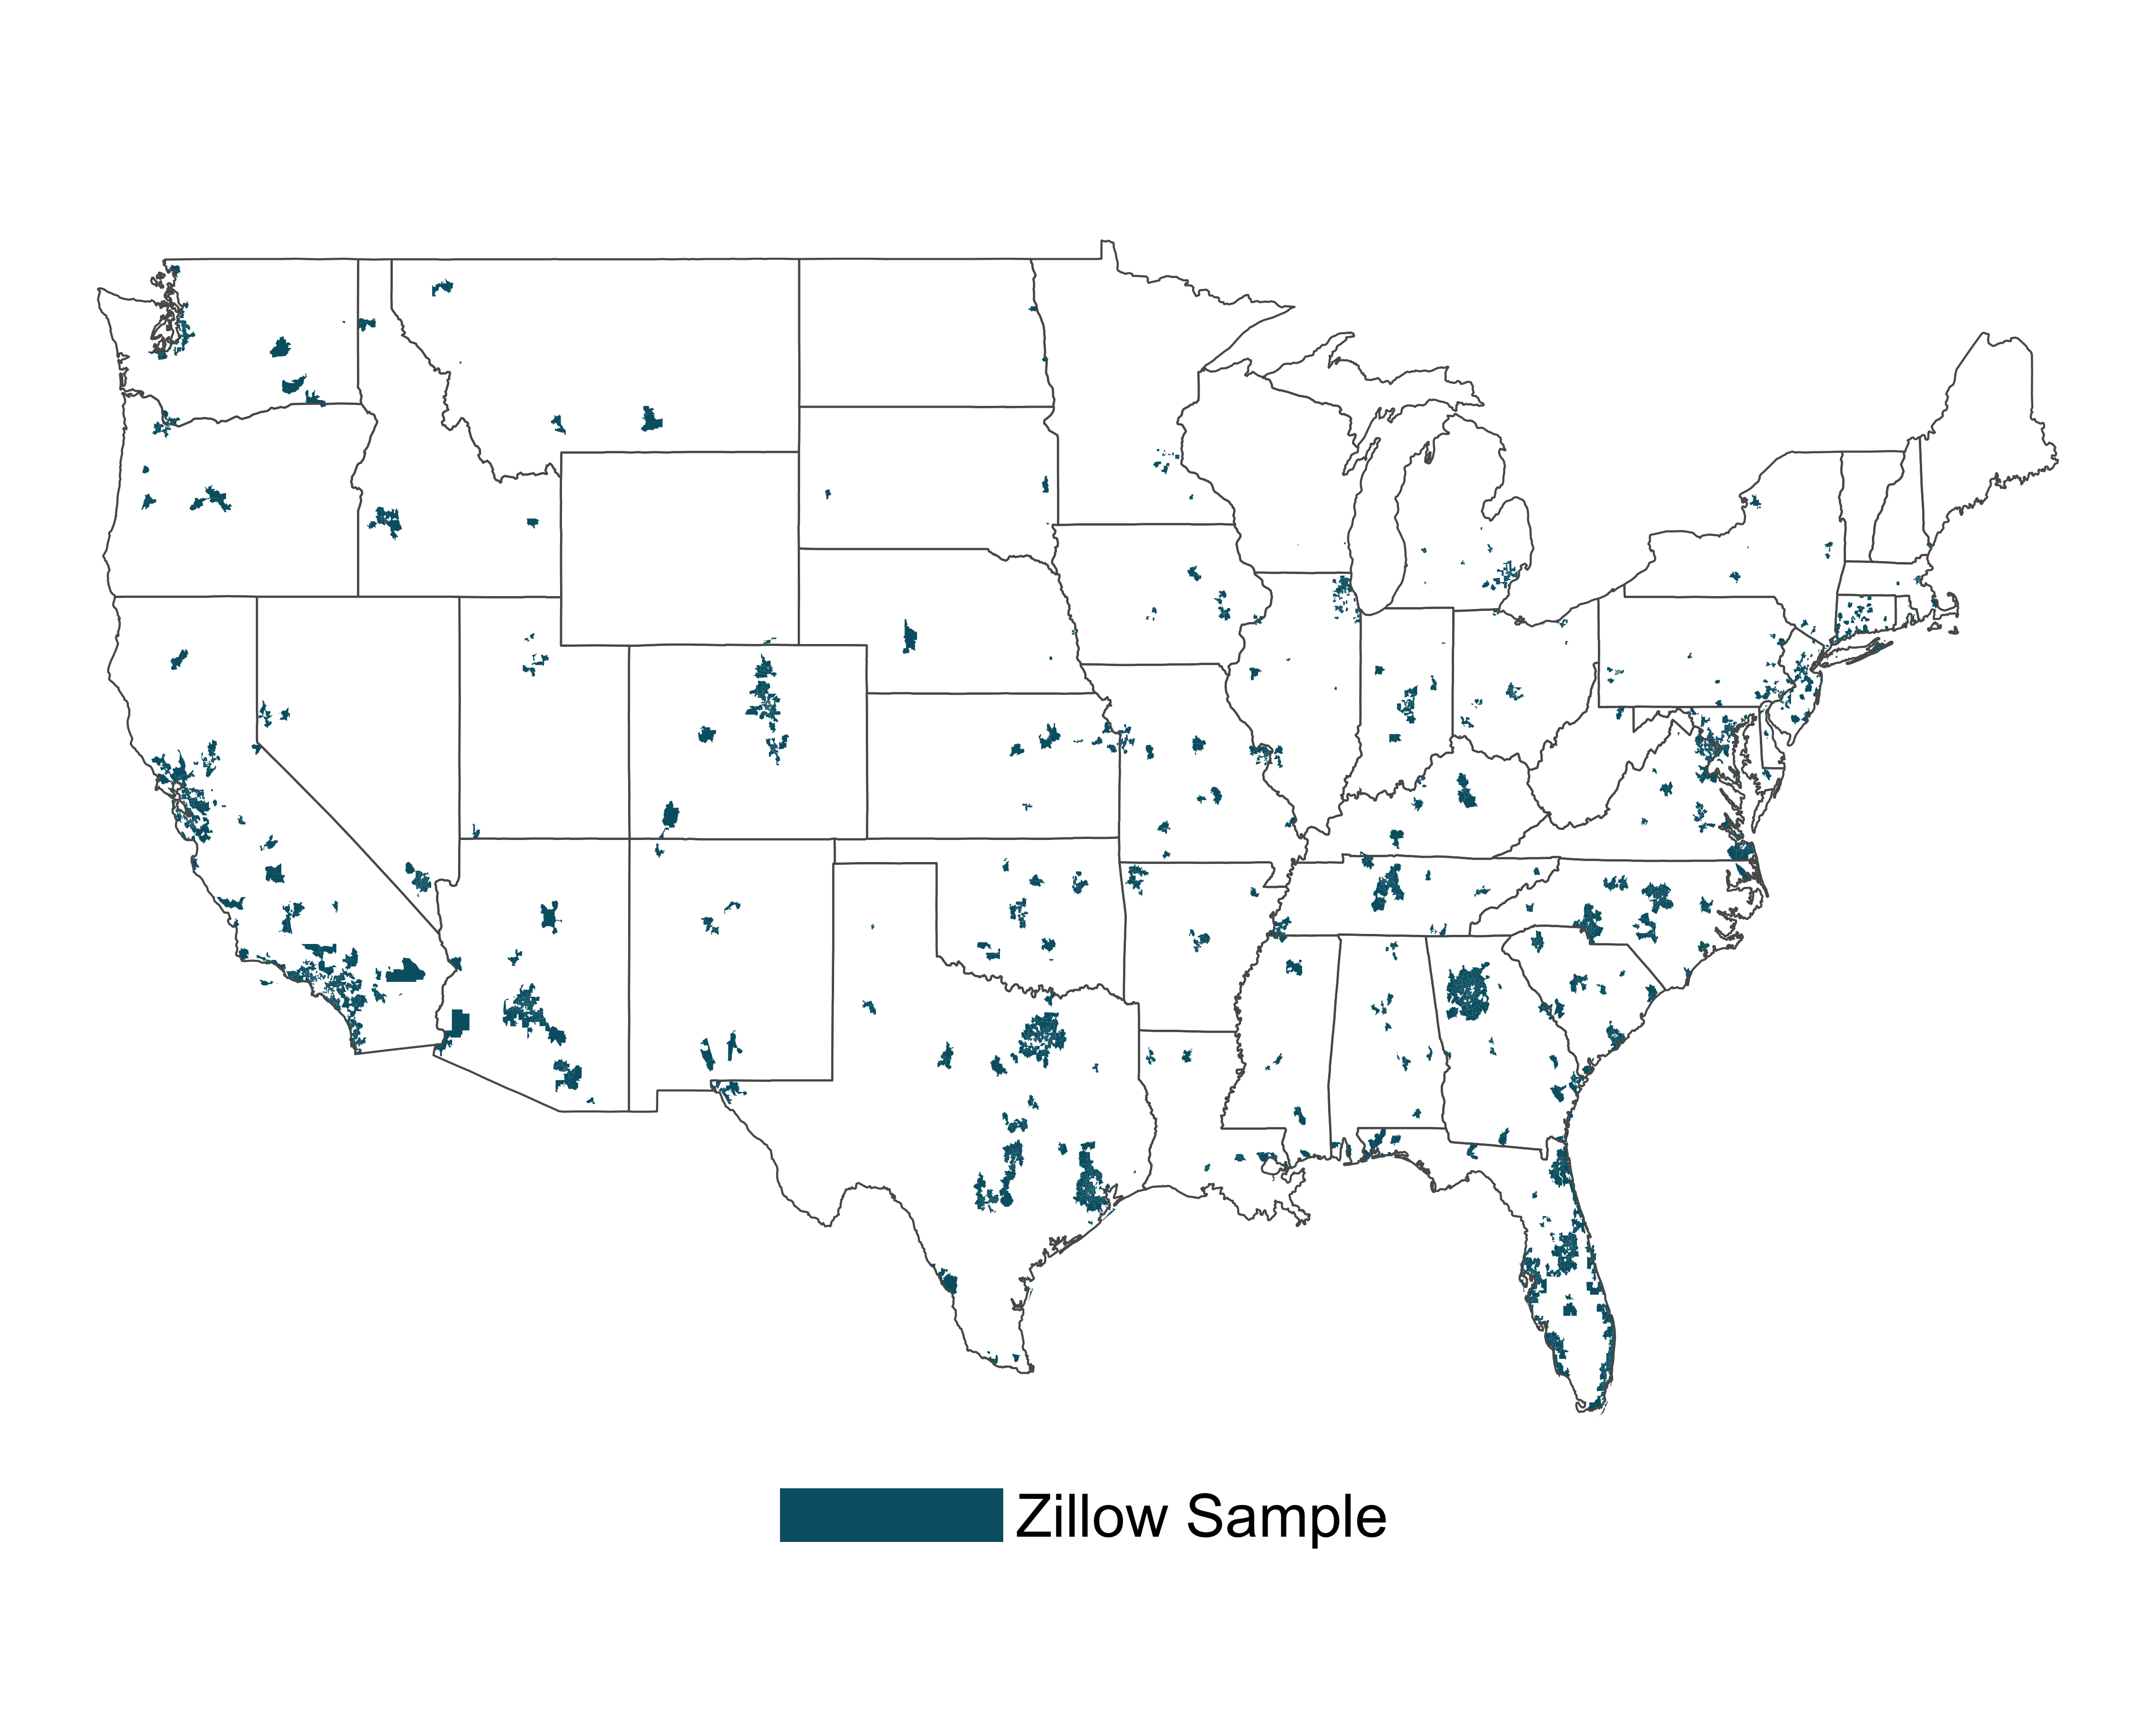
\includegraphics[width = .85\textwidth]{../../analysis/descriptive_maps/output/sample_map.png}
	\end{subfigure}
	\quad 
	\begin{subfigure}[b]{\textwidth}\centering
		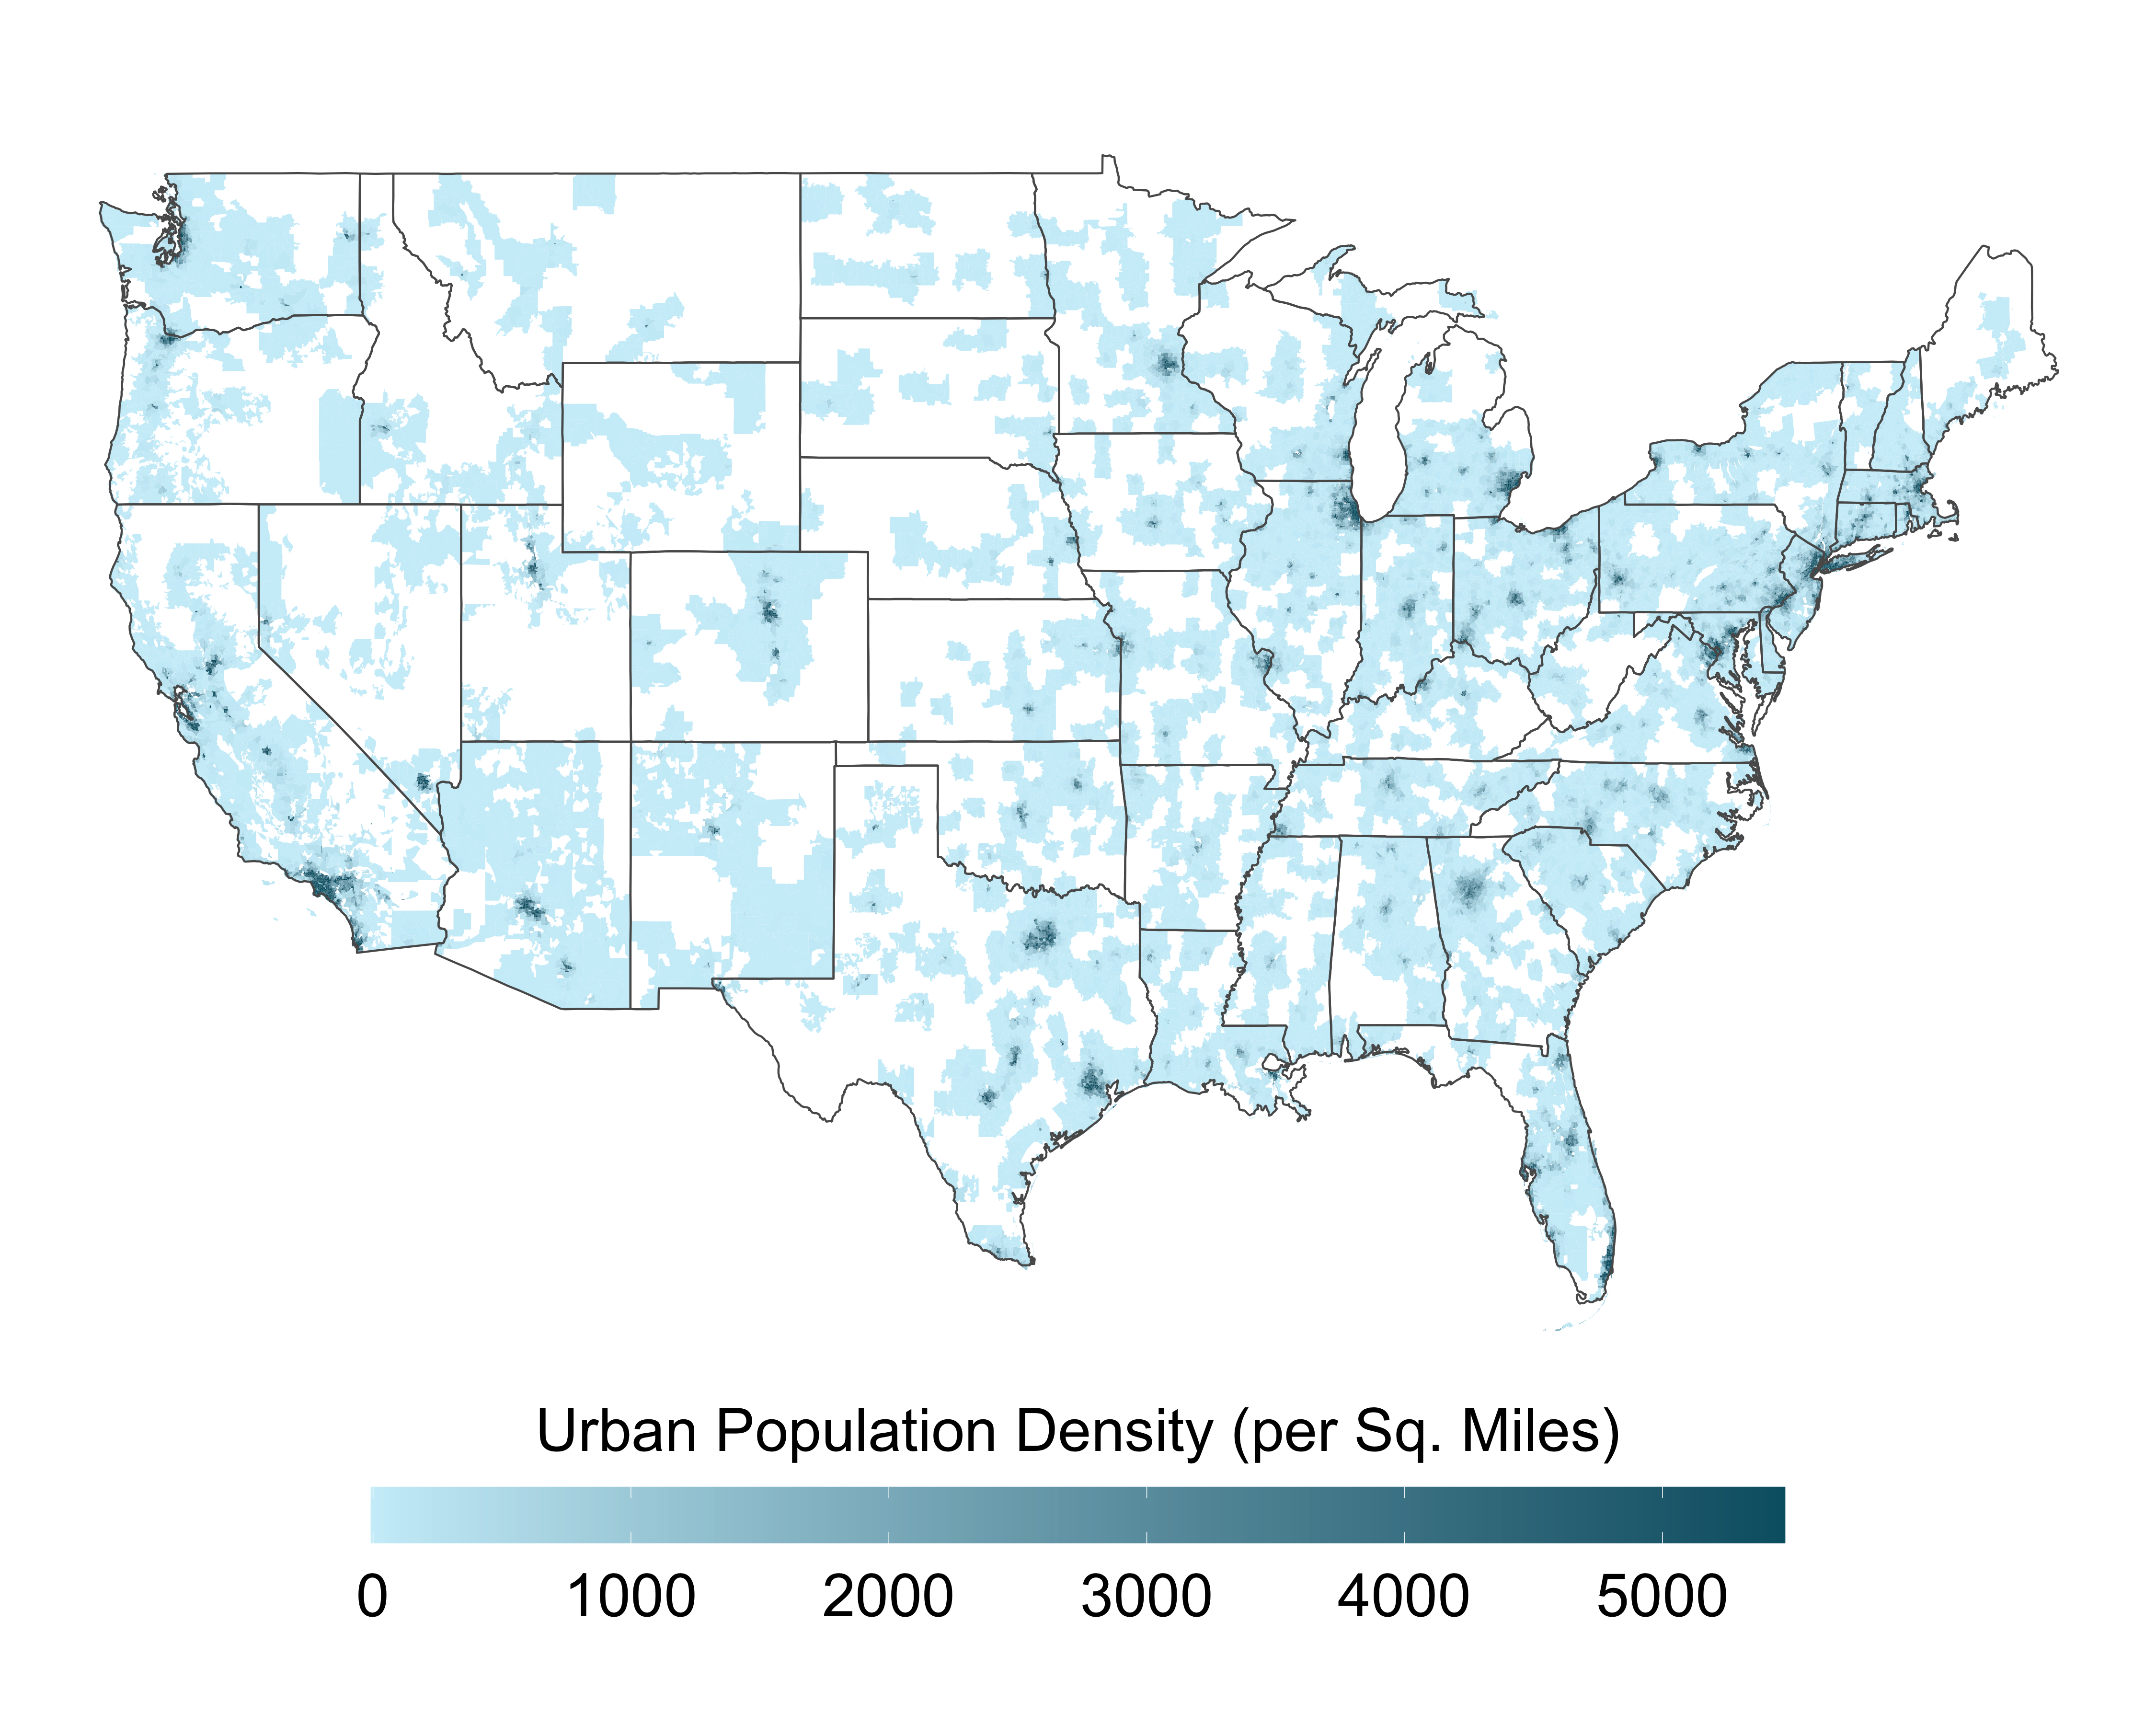
\includegraphics[width = .85\textwidth]{../../analysis/descriptive_maps/output/popurban_density_map.png}
	\end{subfigure}
	\begin{minipage}{.95\textwidth} \footnotesize
	\vspace{2mm} 
	\textit{Notes}: Panel (a) shows the geographical location of the zipcodes present in the Zillow SFCC sample 
	used in the main analysis. Summary statistics are reported in \autoref{tab:desc_stats}, column 3. Panel (b) 
	shows the urban population density for the top 100 metropolitan areas in the U.S. as reported in the 2008-2011 
	ACS. Values are winsorized at the 99 percentile to provide enough graphical variation. 
\end{minipage}

\end{figure}

\begin{figure}[!h]
	\caption{Coefficients of dynamic model for different sets of controls}
	\label{fig:}
	\centering
	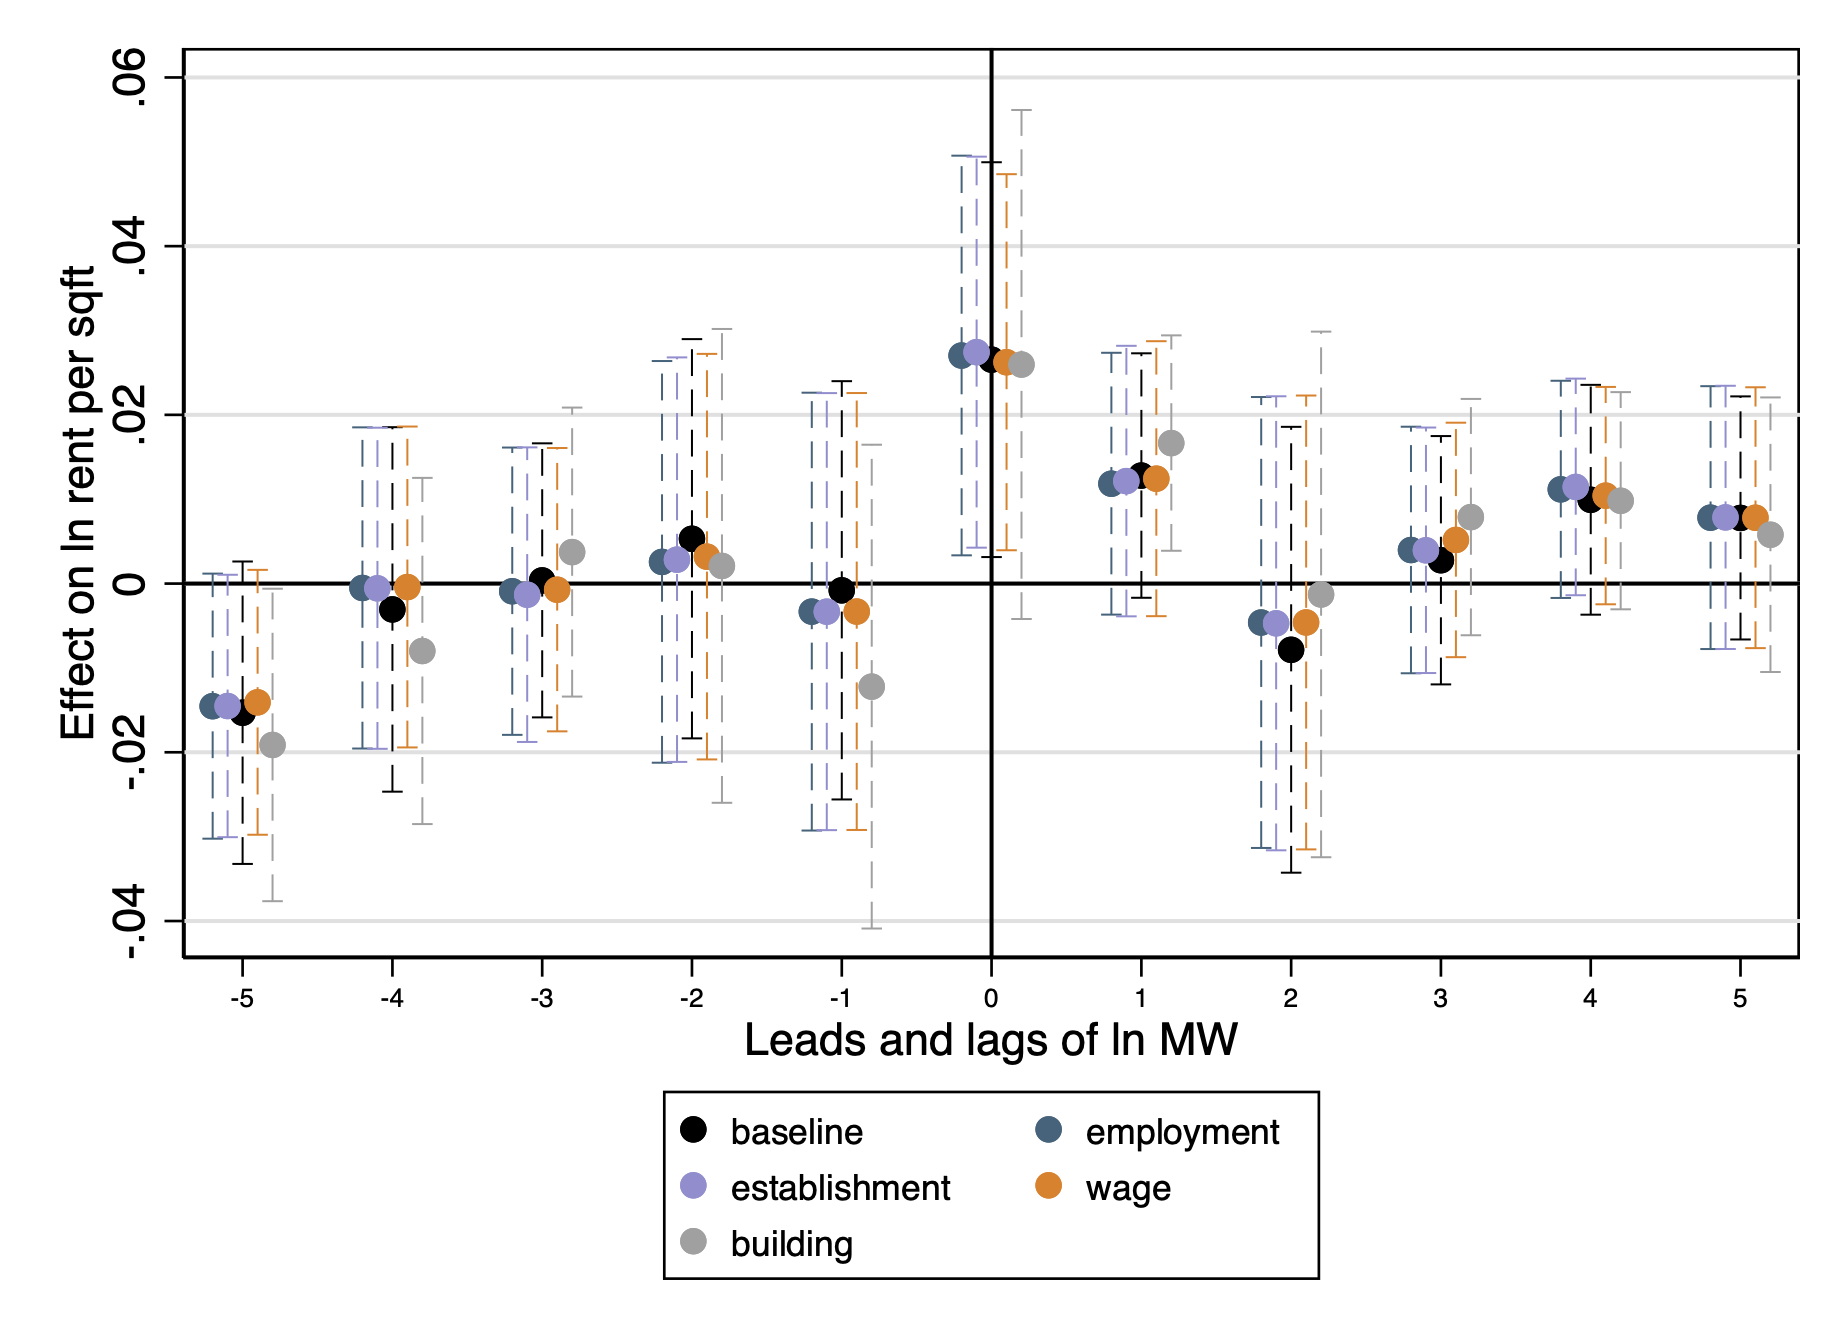
\includegraphics[width = 0.7\textwidth]{../../analysis/first_differences/output/fd_models_control.png}
	\begin{minipage}{.95\textwidth} \footnotesize
		\vspace{2mm} 
		\textit{Notes}: The figure shows the estimated coefficients of the dynamic model defined in 
		equation \autoref{eq:leads_lags} when progressively adding time-varying controls for local shocks. 
		The \textit{baseline} series plots coefficients taken from 
		\autoref{tab:dynamic_lags_leads_main}, column (1). The \textit{employment}, 
		\textit{establishment}, \textit{wage}, and \textit{building} series plot coefficients 
		from \autoref{tab:dynamic_lags_leads_main}, columns (2) to (5) respectively.
		90 percent confidence intervals clustered at the state level reported.
	\end{minipage}
\end{figure}

\begin{figure}[htb!]\centering
	\caption{Placebo Regression with Dependent Variable: (log) Number of SFCCListings for Sale}
	\label{fig:placebo_nlist}
	\includegraphics[width = 0.8\textwidth]{../../analysis/first_differences_nlist/output/fd_placebo.eps}	
	\begin{minipage}{\textwidth}\footnotesize
		\textit{Notes:} The figure shows the estimated coefficients of the dynamic model defined in 
		equation \autoref{eq:leads_lags}. The dependent variable is the difference in the natural logarithm 
		of the number of listings \textit{for sale} in the Single Family, Condos, and Cooperative category in 
		Zillow. The model controls for monthly date fixed effects. In addition, it includes 
		economic controls for the industries ``Professional and business services'', 
		``Information'', and ``Financial activities'' from the QCEW. Wage controls are 
		the difference in the natural logarithm of average weekly wages, employment 
		controls are the difference in the natural logarithm of employment, and 
		establishment count controls refer to the difference in the natural logarithm 
		of number of establishments. Wages and employment vary at the county-month level,
		whereas establishment count varies at the country-quarter level.
		90 percent confidence intervals clustered at the state level reported. 
		
	\end{minipage}
\end{figure}

\begin{figure}[htb!]\centering
	\caption{Comparison between Dynamic Baseline Model, Re weighted Model, and Unbalanced-panel Model}
	\label{fig:dynamic_wgt_unabl_comp}
	\begin{subfigure}[b]{0.75\textwidth}
		\caption{Baseline-Re weighted Models}	
		\includegraphics[width = \textwidth]{../../analysis/first_differences_wgt/output/fd_model_comparison_wgt.eps}
	\end{subfigure}
	\quad
	\begin{subfigure}[b]{0.75\textwidth}
		\caption{Baseline-Unbalanced Models}		
		\includegraphics[width = \textwidth]{../../analysis/first_differences_unbal/output/fd_model_comparison_unbal.eps}
	\end{subfigure}
	\begin{minipage}{\textwidth}\footnotesize
		\textit{Notes:} Panel (a) compares estimated coefficients of the dynamic model defined in 
		equation \autoref{eq:leads_lags} obtained from the baseline sample with those obtained from the
		re-weighted sample. Observations are weighted so as to match the average of the 
		following top-100 CBSA characteristics: ``share of rental houses", ``share of African-American residents", 
		``share of college graduates", and ``median income". All characteristics are obtained from 
		the 2010 U.S. Census and the 2008-2011 ACS. See \autoref{sec:sample_rest} for more details. 
		Panel (b)compares estimated coefficients of the dynamic model defined in 
		equation \autoref{eq:leads_lags} obtained from the baseline sample with those obtained using the 
		unbalanced full sample of Zillow zipcodes. The latter model controls for a ``period of entry $\times$
		zipcode" fixed effect. 
		Both panels additionally show, for each model, the cumulative effect obtained by summing up 
		estimates from a distributed lags only specification. 
		All models control for monthly date fixed effects. All models additionally  
		include economic controls from the industries ``Professional and business services'', 
		``Information'', and ``Financial activities'' from the QCEW. Wage controls are 
		the difference in the natural logarithm of average weekly wages, employment 
		controls are the difference in the natural logarithm of employment, and 
		establishment count controls refer to the difference in the natural logarithm 
		of number of establishments. Wages and employment vary at the county-month level,
		whereas establishment count varies at the country-quarter level.
		90 percent confidence interals clustered at the state level reported. 
	\end{minipage}
\end{figure}


\begin{figure}[h!]\centering
	\caption{Distribution for LODES-based Zipcode-level State shares of Minimum Wage Workers and Residents}
	\label{fig:lodes_share_dist}
	\begin{subfigure}[b]{0.8\textwidth}
	\caption{Share of MW Workers}	
	\includegraphics[width = \textwidth]{../../analysis/first_differences_expmw/output/walall_29y_lowinc_ssh_dist.eps}
	\end{subfigure}
	\quad
	\begin{subfigure}[b]{0.8\textwidth}
		\caption{Share of MW Residents}		
		\includegraphics[width = \textwidth]{../../analysis/first_differences_expmw/output/halall_29y_lowinc_ssh_dist.eps}
	\end{subfigure}
	\begin{minipage}{\textwidth}\footnotesize
		\textit{Notes:} Panel (a) shows the distribution for the zipcode-level state share of MW \textit{workers} identified through the LODES data. 
		Panel (b) shows the distribution for the zipcode-level state share of MW \textit{residents} identified through the LODES data. 
		Both shares are computed dividing the number of workers/residents 29 years old or younger earning less than $\$1,250$/month
		by state totals. For more details on the construction of the shares, see \autoref{sec:experienced_mw}.		
	\end{minipage}	
\end{figure}

\begin{figure}[htb!]\centering
	\caption{Estimated static effect of the MW on rents by workplace and residence of young, low-income workers}
	\label{fig:static_qtl_lodes}
	\begin{subfigure}[b]{.5\textwidth}
		\caption{State share, workplace}
		\includegraphics[width = \textwidth]
		{../../analysis/first_differences_expmw/output/fd_static_heter_walall_29y_lowinc_ssh_st_qtl.eps}
	\end{subfigure}%
	\begin{subfigure}[b]{.5\textwidth}
		\caption{State share, residence}
		\includegraphics[width = \textwidth]
		{../../analysis/first_differences_expmw/output/fd_static_heter_halall_29y_lowinc_ssh_st_qtl.eps}
	\end{subfigure}\\
	\begin{subfigure}[b]{.5\textwidth}
		\caption{Zipcode share, workplace}
		\includegraphics[width = \textwidth]
		{../../analysis/first_differences_expmw/output/fd_static_heter_walall_29y_lowinc_zsh_st_qtl.eps}
	\end{subfigure}%
	\begin{subfigure}[b]{.5\textwidth}
		\caption{Zipcode share, residence}
		\includegraphics[width = \textwidth]
		{../../analysis/first_differences_expmw/output/fd_static_heter_halall_29y_lowinc_zsh_st_qtl.eps}
	\end{subfigure}
	\begin{minipage}{\textwidth}\footnotesize
	\vspace{3mm}	
	\textit{Notes:} The figure reports the estimated static effect of MW on rents for different 
	quartile groups across the distribution of young, low-income workers. More precisely, we estimate
	our static model interacting the MW variable with indicators for quartile groups of zipcode-level 
	characteristics, as explained in \autoref{sec:strategy_heterogeneity}. All figures use counts of 
	workplace and residence of young, low-income workers constructed from LODES data. The top 
	row assigns to each zipcode the share of young, low-income workers that work or live there out 
	of state totals. The bottom row constructs a zipcode share of young, low-income workers out of 
	the working population of that zipcode. All models control for monthly date fixed effects. All 
	models additionally include economic controls from the industries ``Professional and business 
	services'', ``Information'', and ``Financial activities'' from the QCEW, as specified throughout
	the paper. 90 percent confidence intervals clustered at the state level reported. 
\end{minipage}
\end{figure}

\begin{figure}[!h]
	\centering
	\caption{Estimated Impact of changes in Experienced MW on changes in Rents - Dynamic DiD model}
	\label{fig:expmw_dynamic}
	\includegraphics[width = .9\textwidth]{../../analysis/first_differences_expmw/output/fd_model_comparison_expmw.eps}
	\begin{minipage}{.9\textwidth}\footnotesize
		\textit{Notes:} The figure compares estimated coefficients of the dynamic model defined in 
		equation \autoref{eq:leads_lags} obtained from the baseline sample with those obtained when 
		replacing the statutory MW with the experienced MW as main explanatory variable. 
		The plot additionally shows, for each model, the cumulative effect obtained by summing up 
		estimates from a distributed lags only specification. 
		All models control for monthly date fixed effects. All models additionally  
		include economic controls from the industries ``Professional and business services'', 
		``Information'', and ``Financial activities'' from the QCEW. Wage controls are 
		the difference in the natural logarithm of average weekly wages, employment 
		controls are the difference in the natural logarithm of employment, and 
		establishment count controls refer to the difference in the natural logarithm 
		of number of establishments. Wages and employment vary at the county-month level,
		whereas establishment count varies at the country-quarter level.
		90 percent confidence intervals clustered at the state level reported. 
	\end{minipage}
\end{figure}

\clearpage
%%%%%%%%%%%%%%%%%%%%%%%%%%%%%%%%%%%%%%%%%%%%%%%%%%%%%%%%%%%%%%%%%%%%%%%%%%%%%%%%%
\section{A Direct test of the Impact of Minimum Wage on Time-Varying Economic Controls}\label{sec:app_econ_control}
In all the model specifications presented in the paper, we use county-level data from the QCEW 
to control for the local business cycle. However, a potential concern in using local 
economy data may arise if changes in the MW have a \textit{direct} impact on such quantities. This 
would lead the treated and control group be systematically different \parencite{AngristPischke2009}. 

To avoid the ``bad controls" problem, while at the same time including control variables that truly proxy for the 
local economic conditions, we select QCEW county-level time-series for the following industries: "Professional 
and Business Services"; "Information"; and "Finance". According to the Bureau of Labor Statistics (BLS), 
in 2019 such industries accounted for $3.5$, $1$, and $1.2$ percent of the total MW workers respectively, making them 
unlikely to be direcly impacted by MW legislation.\footnote{See the 2020 BLS report on minimum wage workers.} For each 
industry, we observe county-month employment, and county-quarter average weekly wages and establishment count. 

To provide further evidence on the chosen controls' validity, we use them as left-hand side variable in a dynamic DiD
model. The presence of significant pre-treatment trends would suggest how MW react to local economic shocks and
cast doubts on the identification strategy introduced in \autoref{sec:empirical_strategy}. 

QCEW data are aggregated at the county-level, hence preventing us to estimate \autoref{eq:leads_lags}. We therefore 
aggregate MW zipcode-month information at the county-month level by taking, for each period, 
the weighted average of MW levels in each zipcode associated with a given county, using the number of housing units 
as weights. For counties without city-level ordinances, this would simply reflect the state- or county-level MW. Since 
QCEW provides county-month employment data, we are able to estimate the following regression model: 

\begin{equation}
	\label{eq:dynamic_econ_cont_month}
	\Delta y_{ct} = \delta_{t} + \sum\limits_{r=-s}^{s} \beta_r \Delta \underline{w}_{c,t+r} + \Delta \nu_{ct}
\end{equation}

where $y_{ct}$ is the (log) employment in county $c$ in month $t$. The exogeneity 
assumption requires that  $E \left[ \Delta \nu_{ct} | \delta_t, \{ \Delta \underline{w}_{c,t+r} \} \forall r \right] =  0$ 

As for wages and establishment count, the data
is aggregated at the county-quarter level. We hence estimate the impact of the average MW change in a quarter 
over the average rent change. This amounts to running the following regression: 

\begin{equation}
	\label{eq:dynamic_econ_cont_quarter}
	\overline{\Delta y}_{cq} = \overline{\delta}_q +  \sum\limits_{r=-s}^{s} \rho_r \overline{\Delta \underline{w}}_{c,q+r} + \overline{\Delta \nu}_{ct}
\end{equation}

where $\overline{\Delta x}_{cq} = \frac{1}{3} \Delta x_{cq}$ (the quarterly average). Notice that estimating \autoref{eq:dynamic_econ_cont_month} 
and \autoref{eq:dynamic_econ_cont_quarter} is equivalent because the average change over a quarter is a linear combination of 
monthly changes.

ADD PLOTS

%%%%%%%%%%%%%%%%%%%%%%%%%%%%%%%%%%%%%%%%%%%%%%%%%%%%%%%
\section{A toy model of the local housing market}\label{sec:model}

We build a simple model that is used to build a benchmark estimate of the effect of MW
policies on rents.

\subsection{Model set-up}

We focus on the supply and demand of housing in a given zipcode. Consider an environment with 
an exogenously given continuum of households in each zipcode divided in two groups: minimum wage 
and non-minimum wage households (HH). The former are fully affected by the MW, whereas the latter 
are not affected at all.

On the supply side, we denote by $H$ the continuous measure of housing units available for rent 
in the zipcode. We assume that units are homogeneous, and can be rented at the a rent of $r$. The 
supply of housing $H(r)$ is assumed to be increasing in rents $r$, so that $H'(r) > 0$.

Let us move to the demand side. Households receive monthly a income, which we denote by 
$\underline{w}$ and $w$ for MW HH and non-MW households, respectively. Demand for housing is given 
by $\underline{H}(r, \underline{w})$ and $\overline{H}(r, w)$ for each household type. We make two 
standard assumptions on these objects: (i) the demand of housing is downward sloping (i.e., 
$\underline{H}_r(r, \underline{w}) < 0$ and $\overline{H}_r(r, w) < 0$); and (ii) the demand for 
housing is increasing in income (i.e., $\underline{H}_w(r, \underline{w}) > 0$ and $\overline{H}_w(r, 
w) > 0$)


\subsection{Equilibrium and the elasticity of rents to the minimum wage}

Equilibrium rents $r^*$ are such that local housing supply is equated to local housing demand. 
Formally,

\begin{equation*}\label{eq:model-eq}
H(r) =  \underline{H}(r, \underline{w}) + \overline{H}(r, w) \ .
\end{equation*}

We are interested in the elasticity of equilibrium rents $r^*$ to the minimum wage $\underline{w}$, 
which we denote by $\rho$. The implicit function theorem applied on the above equation yields

\begin{equation}\label{eq:model-elasticity}
\rho := \frac{d \ln r^*}{d \ln \underline{w}} 
= \frac{\underline{w} \ \underline{H}_w}
{r\  H'(r) - r \ \underline{H}_r - r \ \overline{H}_r} \ ,
\end{equation}
where we denote partial derivatives with sub-indexes.

Note that, since $\underline{H}_r < 0$ and $\overline{H}_r < 0$, the above expression is always 
positive. When the MW increases the local housing market moves to a new equilibrium with higher 
rents. The magnitude of the elasticity is driven by the relative magnitudes of the earnings of 
minimum wage workers ($\overline{w}$) and rents ($r$), and the slopes of the different 
functions in equilibrium. For instance, a higher response of housing demand to the minimum wage 
change ($\underline{H}_w$) would result in a higher elasticity.